\documentclass[11pt]{article}
\usepackage[letterpaper,margin=1in]{geometry}
\usepackage{amsmath,amssymb,amsfonts}
\usepackage{booktabs,tabularx,array,multirow}
\usepackage{graphicx,float,caption}
\usepackage{xcolor}
\usepackage{microtype}
\usepackage{enumitem}
\usepackage{cite}
\usepackage[hidelinks]{hyperref}
\usepackage{url}
\usepackage{xspace}

\definecolor{cbadred}{HTML}{C0392B}
\definecolor{modelblue}{HTML}{2874A6}
\definecolor{cfbagreen}{HTML}{17A589}
\definecolor{softgray}{HTML}{F3F5F7}
\newcommand{\method}{MD-CBAD-DQN\xspace}
\newcommand{\R}{\mathbb{R}}
\DeclareMathOperator{\clip}{clip}

\title{\textbf{MD-CBAD-DQN: Model-Driven Counterfactual Bellman Advantage Distillation for Long-Term Satellite-Ground Task Scheduling}}
\author{
Bocheng Yang$^{1}$, Lujie Zheng$^{1}$, Jian Liu$^{1,2,*}$, and Bo Chen$^{1,*}$\\[3pt]
\small $^{1}$School of Aerospace, Harbin Institute of Technology (Shenzhen), Shenzhen 518055, China\\
\small $^{2}$Guangxi Key Laboratory of Precision Navigation Technology and Application,\\[-2pt]
\small Guilin University of Electronic Technology, Guilin 541004, China\\
\small $^{*}$Correspondence: liujian2024@hit.edu.cn; hitchenbo@hit.edu.cn
}
\date{}

\begin{document}
\emergencystretch=2em
\maketitle
\newcommand{\CBADvsDQNMinPct}{1.48\%\xspace}
\newcommand{\CBADvsDQNMaxPct}{2.95\%\xspace}
\newcommand{\CBADvsCFBALinkDiff}{-3.33\xspace}
\newcommand{\CBADvsCFBALinkCI}{[-6.20, -0.46]\xspace}
\newcommand{\StaticArgminCost}{179.68\xspace}
\newcommand{\StaticCBADCost}{208.49\xspace}
\newcommand{\ReducedArgminCost}{202.08\xspace}
\newcommand{\ReducedCBADCost}{222.62\xspace}
\newcommand{\NominalDQNCost}{329.21\xspace}
\newcommand{\NominalCFBACost}{324.72\xspace}
\newcommand{\NominalCBADCost}{324.03\xspace}

\newcommand{\PhysicalCBADMinPct}{1.03\%\xspace}
\newcommand{\PhysicalCBADMaxPct}{3.38\%\xspace}
\newcommand{\SensitivityMinPct}{1.81\%\xspace}
\newcommand{\SensitivityMaxPct}{7.43\%\xspace}
\newcommand{\PhysicalCorrDataWork}{0.660\xspace}
\newcommand{\MPCNominalPlanningMs}{4.70\xspace}
\newcommand{\MPCNominalCost}{90.81\xspace}
\newcommand{\PhysicalNominalDQNCost}{79.92\xspace}
\newcommand{\PhysicalNominalCBADCost}{77.22\xspace}
\newcommand{\CenteringSupportedCount}{0\xspace}
\newcommand{\PhysicalAuditTasks}{20,000\xspace}


\begin{abstract}
Satellite-ground scheduling is temporally coupled because a locally inexpensive action can consume resources needed by later tasks. A standard deep Q-network (DQN) nevertheless trains only the executed action, even when an analytical model can evaluate every one-step alternative. We introduce \method, which constructs model-based Bellman targets for all processing modes and distills their centered within-state advantages. The factual update, network, replay, exploration schedule, and standard DQN target remain unchanged. To address physical validity, tasks are generated from correlated data-volume and workload primitives; heat, energy, latency, and transmitted volume are derived rather than independently sampled. Five independently trained models were evaluated on shared traces in seven regimes and eight prespecified parameter envelopes. Against standard DQN, \method reduced mean cost by \PhysicalCBADMinPct--\PhysicalCBADMaxPct across all five fully coupled regimes, with every paired 95\% interval below zero. The effect remained supported under all sensitivity profiles. An exact four-step receding-horizon comparator and coupling controls delimit the planning claim: analytical planning is preferable when coupling is absent or weak, whereas the learned policies perform better under longer resource carryover. The physical-consistency study supports full-action counterfactual supervision, but it does not isolate a significant incremental effect of centering over uncentered CFBA.
\end{abstract}

\noindent\textbf{Keywords:} satellite edge computing; task scheduling; model-driven reinforcement learning; counterfactual supervision; Bellman advantage distillation.

\begin{figure}[H]
\centering
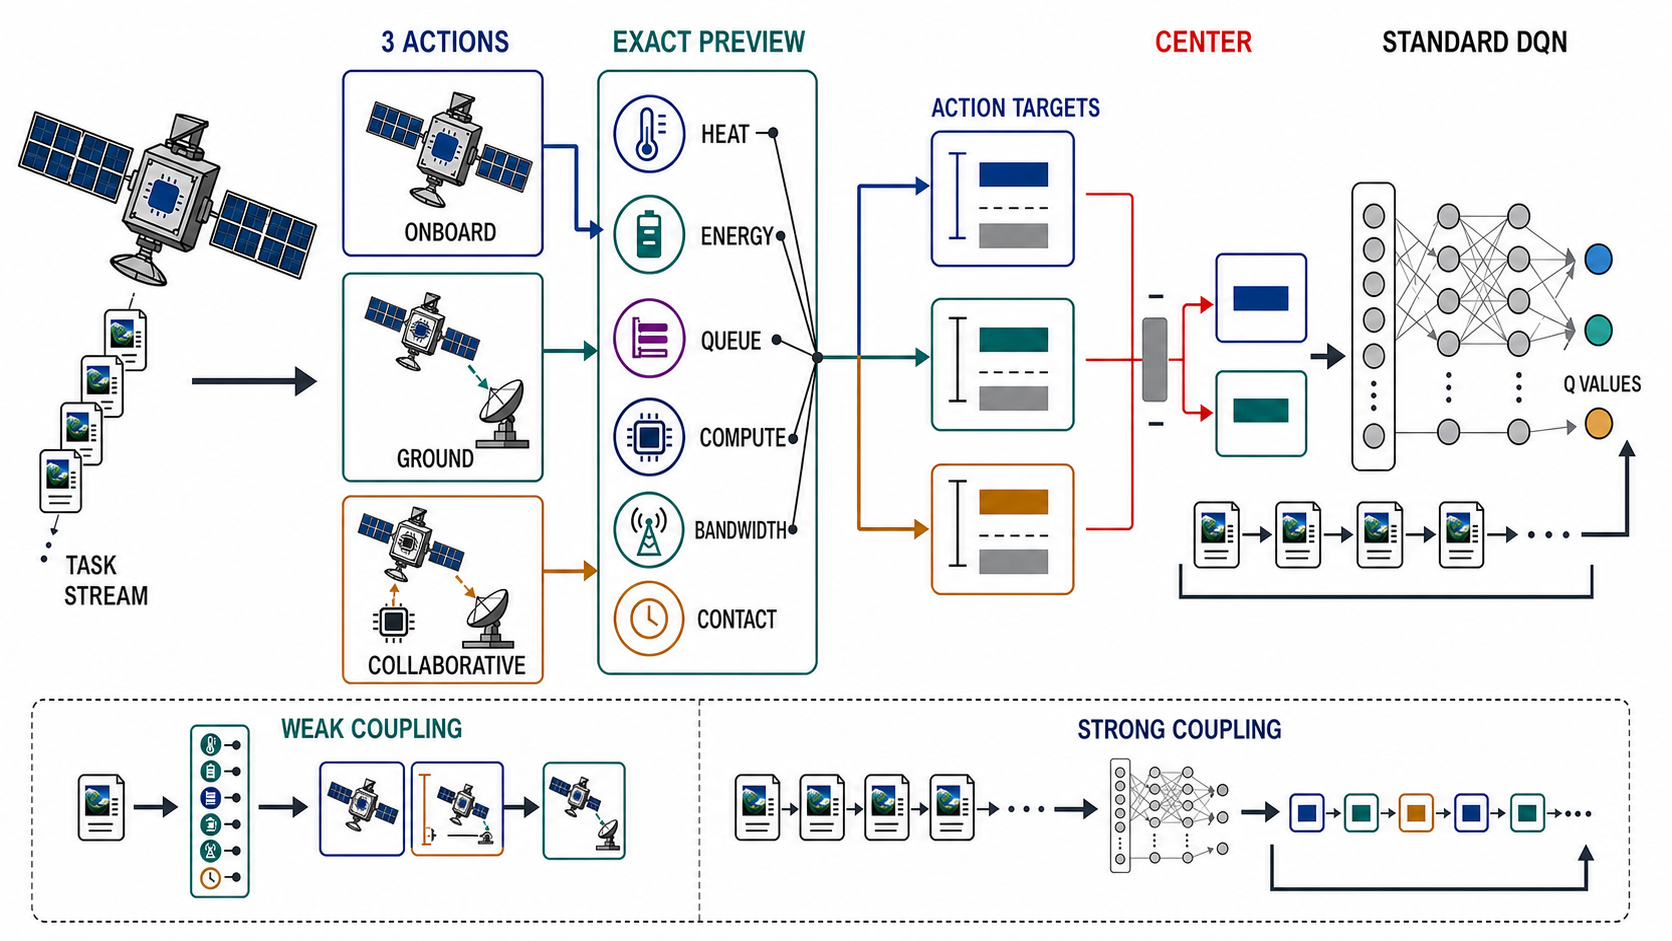
\includegraphics[width=0.98\textwidth,height=0.42\textheight,keepaspectratio]{figures/ai/fig_graphical_abstract_arial.png}
\caption{Graphical overview of \method. Exact analytical previews expose the immediate cost and six post-action resources for all three scheduling actions. Centering the resulting Bellman targets isolates action-relative supervision while the factual standard-DQN update remains unchanged. The illustration is conceptual and encodes no quantitative results.}
\label{fig:graphical}
\end{figure}

\section{Introduction}

Earth-observation and communication satellites increasingly execute perception and decision workloads in orbit. Compact networks can reduce downlink demand and response latency under constrained onboard resources~\cite{9925218,10107454,10378728,10440355,10423050}. Yet onboard execution consumes heat, energy, and compute capacity, while ground offloading consumes contact time and bandwidth. A scheduler must therefore choose among onboard execution, complete offloading, and collaborative preprocessing.

Existing schedulers optimize constellation coordination, observation plans, service placement, deadlines, makespan, or energy use~\cite{RN8,RN9,RN10,RN20,RN22,RN23,RN27,RN28}. The present decision instead changes six resources that persist across task arrivals. These resources are heat, energy, queue occupancy, compute utilization, bandwidth, and remaining contact. Consequently, minimizing a known immediate cost need not minimize episode cost.

Standard DQN~\cite{mnih2015human,watkins1992q} learns one Bellman target from each factual tuple $(s_t,a_t,r_t,s_{t+1})$. Here, the resource equations can also evaluate every unexecuted action without advancing the environment or revealing later tasks. The unresolved question is how to use these exact alternatives while preserving a controlled standard-DQN comparison. Absolute counterfactual targets provide more supervision, but their common state-value offset does not affect action selection.

We address this question with \method. The method previews every action, forms standard target-network Bellman targets, and centers predicted and target values within each state. It then distills the resulting action advantages while the factual Huber loss anchors the absolute Q scale. Counterfactual previews are restricted to training.

Our contributions are:

\begin{enumerate}[leftmargin=1.6em]
    \item We formulate three satellite-ground processing modes as a 21-dimensional sequential problem and derive coupled heat, energy, latency, and transmission descriptors from common task primitives.
    \item We introduce centered counterfactual Bellman advantage distillation, which uses exact full-action outcomes to supervise the action gaps that determine scheduling decisions.
    \item We isolate this mechanism through matched factual, uncentered full-action, and centered updates, then test it against a four-step model-based planner across seven regimes and eight parameter envelopes.
\end{enumerate}

\section{Related Work and Novelty Positioning}

\subsection{Satellite-ground scheduling}

Satellite schedulers cover constellation coordination, observation planning, service placement, and energy-aware offloading~\cite{RN8,RN9,RN10,RN20,RN22,RN23,RN27,RN28}. Our setting combines an explicit cost for every action with resource carryover between task arrivals. The one-step objective is therefore observed rather than hidden. Learning is justified only when present actions change future feasibility.

\subsection{Model use and counterfactual learning}

Dyna established predicted experience for value learning and planning~\cite{sutton1991dyna}. Counterfactual data fusion and causal augmentation construct transitions under structural assumptions~\cite{forney2017counterfactual,armengol2024caiac}. Counterfactual credit assignment instead separates action influence from future randomness~\cite{mesnard2021counterfactual}. Recent work also studies multi-action generative interfaces and joint quantities across action outcomes~\cite{kaya2026joint}. Counterfactual information in reinforcement learning is therefore not new by itself.

Advantage learning widens action gaps through modified operators~\cite{bellemare2016gap}, whereas \method preserves the standard Bellman operator. It adds centered targets from an exact domain model but does not synthesize replay trajectories. Each alternative shares the current task and exogenous next task, while only six endogenous resources change. Our novelty claim is consequently narrow. We claim this full-action, centered auxiliary objective and its scheduling application, not counterfactual simulation or advantage learning in general.

\section{System Model and Immediate-Cost Quantification}
\label{sec:system}

At task arrival $t$, a satellite selects one of three actions:
\begin{equation}
\mathcal A=\{\alpha_s,\alpha_g,\alpha_{s\&g}\},
\end{equation}
where $\alpha_s$ executes onboard and downlinks the result, $\alpha_g$ downlinks the complete input for ground execution, and $\alpha_{s\&g}$ performs onboard preprocessing followed by ground execution.

\begin{figure}[H]
\centering
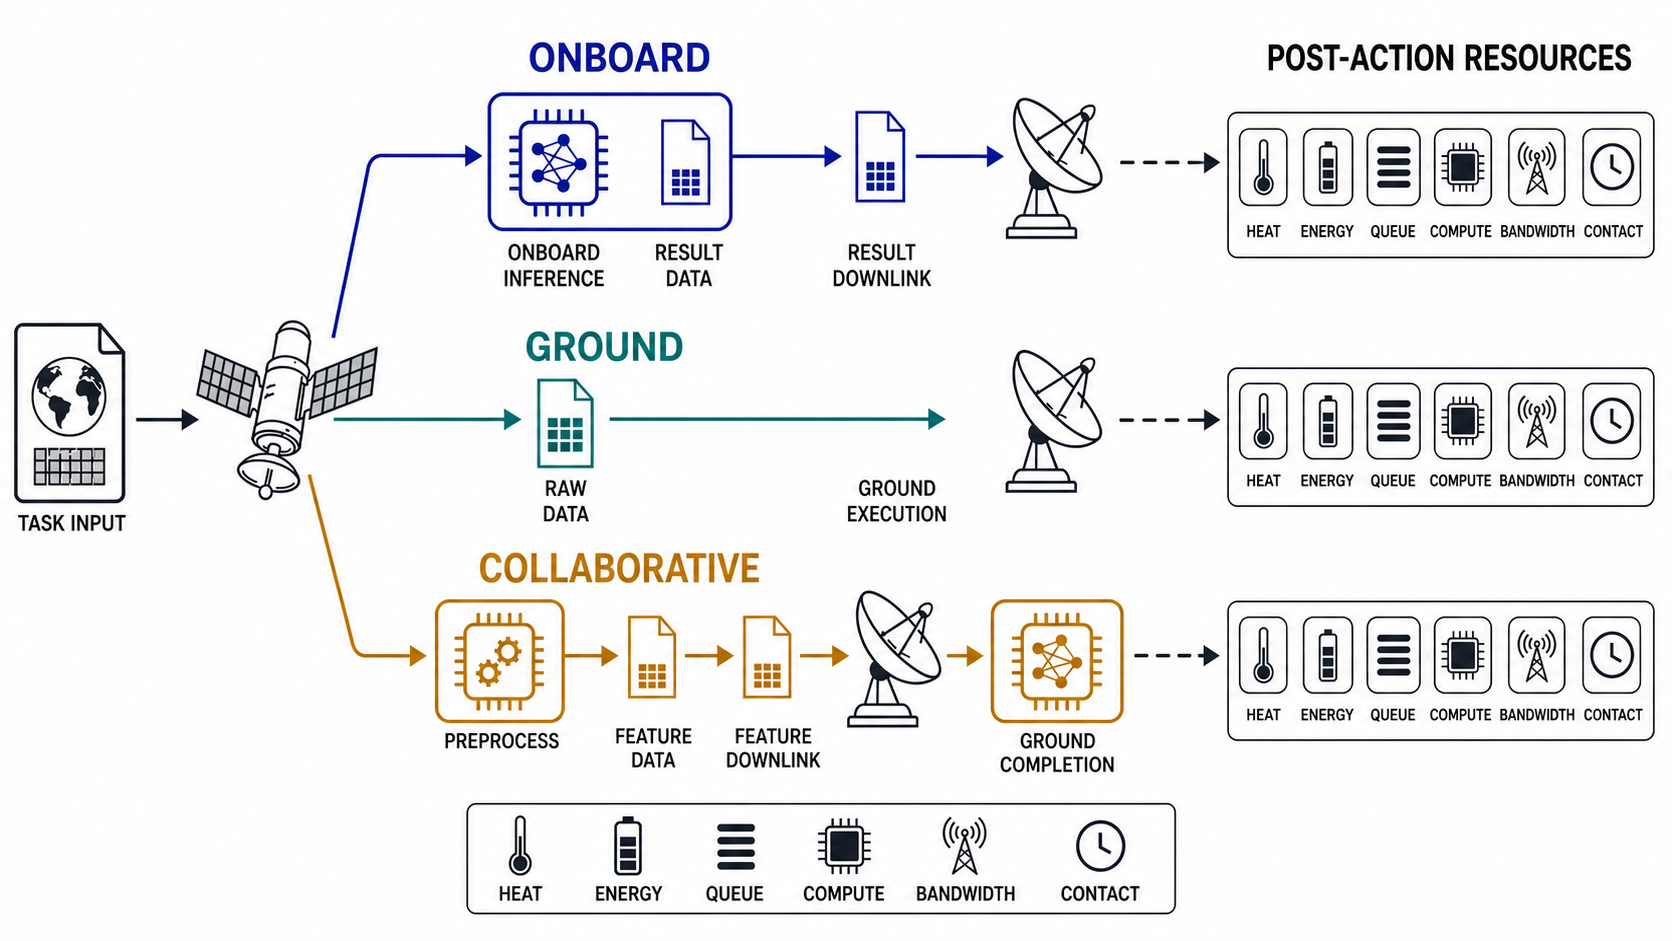
\includegraphics[width=0.98\textwidth,height=0.42\textheight,keepaspectratio]{figures/ai/fig_system_modes_arial.png}
\caption{Three satellite-ground processing pathways. Each arriving task is executed onboard, transferred for ground execution, or preprocessed collaboratively before ground completion. The analytical transition model returns the immediate cost and the post-action heat, energy, queue occupancy, compute utilization, bandwidth, and remaining contact.}
\label{fig:system}
\end{figure}

\subsection{Cost factors}

The model combines five physical or operational factors using dimensionless coefficients $\rho$ and relative weights $\omega$. Explicit factors make the reward auditable and preserve the original cost derivations.

\subsubsection{Thermal cost}

\begin{equation}
C_1=
\begin{cases}
\rho_{heat}\omega_{heat}\tan\!\left(\dfrac{\pi}{2}\dfrac{Q}{Q_{\max}}\right),&Q<Q_{\max},\\[5pt]
+\infty,&Q\ge Q_{\max}.
\end{cases}
\label{eq:heat}
\end{equation}
The tangent barrier grows rapidly near the allowable heat threshold. This form prevents thermal safety from being traded linearly against latency~\cite{karkadakattil2025ai}.

\subsubsection{Computational load}

\begin{equation}
C_2=\rho_{comp}\omega_{comp}\,\mathrm{FLOPs}.
\label{eq:compute}
\end{equation}
FLOPs are measured in mega floating-point operations and represent the finite onboard compute budget.

\subsubsection{Processing and transmission latency}

\begin{equation}
C_3=\rho_{time}\left(\omega_{proc}t^{proc}+\omega_{trans}t^{trans}\right).
\label{eq:latency}
\end{equation}
The two terms separate execution delay from communication delay. Available bandwidth and contact duration modulate the latter~\cite{abdulkarim2025multi}.

\subsubsection{Co-location overhead}

\begin{equation}
C_4=\rho_{coloc}\omega_{coloc}f(n),
\label{eq:colocation}
\end{equation}
where $f(n)$ grows with the number of concurrently resident tasks. This term represents contention among co-located services~\cite{10589437}.

\subsubsection{Bandwidth occupancy}

\begin{equation}
C_5=
\begin{cases}
\rho_{bw}\omega_{bw}\tan\!\left(\dfrac{\pi}{2}\dfrac{B}{B_{\max}}\right),&B<B_{\max},\\[5pt]
+\infty,&B\ge B_{\max}.
\end{cases}
\label{eq:bandwidth}
\end{equation}
The nonlinear penalty represents increasing scarcity near the downlink capacity limit~\cite{zhang2024dynamic}.

\subsection{Action-specific immediate costs}

For onboard execution, all five factors apply:
\begin{align}
\mathrm{Cost}_s={}&\rho_{heat}\omega_{heat}\tan\!\left(\frac{\pi Q_s}{2Q_{\max}}\right)
+\rho_{comp}\omega_{comp}\mathrm{FLOPs}_s \notag\\
&+\rho_{time}\left(\omega_{proc}t_s^{proc}+\omega_{trans}t_s^{trans}\right)
+\rho_{coloc}\omega_{coloc}f(n)_s \notag\\
&+\rho_{bw}\omega_{bw}\tan\!\left(\frac{\pi B_s}{2B_{\max}}\right).
\label{eq:onboard}
\end{align}

For complete ground offloading, the spacecraft incurs transmission heat, latency, and bandwidth occupancy, while the server cost collects ground computation, heat, and processing delay:
\begin{align}
\mathrm{Cost}_g={}&\rho_{heat}\omega_{heat}\tan\!\left(\frac{\pi Q_g}{2Q_{\max}}\right)
+\rho_{time}\omega_{trans}t_g \notag\\
&+\rho_{bw}\omega_{bw}\tan\!\left(\frac{\pi B_g}{2B_{\max}}\right)
+\mathrm{cost}_{ground\_server}.
\label{eq:ground}
\end{align}

Collaborative processing adds onboard preprocessing and transmission components:
\begin{align}
\mathrm{Cost}_{s\&g}={}&\rho_{heat}\omega_{heat}
\tan\!\left(\frac{\pi(Q^{pre}_{s\&g}+Q^{trans}_{s\&g})}{2Q_{\max}}\right) \notag\\
&+\rho_{time}\left(\omega_{pre}t^{pre}_{s\&g}+\omega_{trans}t^{trans}_{s\&g}\right)
+\rho_{comp}\omega_{comp}\mathrm{FLOPs}_{s\&g} \notag\\
&+\rho_{bw}\omega_{bw}\tan\!\left(\frac{\pi B_{s\&g}}{2B_{\max}}\right)
+\mathrm{cost}_{ground\_server}.
\label{eq:hybrid}
\end{align}

At decision time, $B_{\max}$ becomes the available downlink capacity. Effective latency depends on link quality and utilization, while co-location depends on queue occupancy. The same task can therefore incur different costs under different inherited resource states.

\subsection{Physically coupled task and communication generator}

The revised simulator does not sample heat, workload, data volume, and latency independently. It first draws correlated latent variables $(v_t,w_t)$ with correlation parameter 0.68 and maps them through a logistic transform to raw data volume $D_t\in[8,64]$ Mbit and workload $W_t\in[0.25,4.0]$ GFLOP. Result and collaborative-feature volumes are
\begin{equation}
D_t^{res}=r_tD_t,\quad r_t\in[0.01,0.05],\qquad
D_t^{feat}=f_tD_t,\quad f_t\in[0.08,0.30].
\end{equation}
The implementation enforces $D_t^{res}\le D_t^{feat}\le D_t$. A workload-dependent fraction $p_t\in[0.20,0.45]$ is processed onboard in the collaborative mode. Given onboard and ground rates $R_s=4$ and $R_g=80$ GFLOP s$^{-1}$, processing time is derived as $W/R$, rather than sampled separately. Compute power rises monotonically from 4 to 20 W with workload; compute heat is 0.78 times compute energy. Transmission time is data volume divided by the effective return rate
\begin{equation}
R_t^{link}=2.2+217.8b_t\quad\text{Mbit s}^{-1},
\end{equation}
and transmission heat is 0.55 times transmit energy. These values are engineering envelopes, not fitted flight distributions. Their scale is consistent with the range of modern SmallSat computing-system power reported by NASA and with NASA ground-network examples spanning 2.2 Mbit s$^{-1}$ S-band to 220 Mbit s$^{-1}$ X-band returns~\cite{nasa2026avionics,nasa2026ground}. The bounded data-reduction factors represent the bandwidth-reduction role of onboard image compression, not a claim about one instrument-specific codec~\cite{ccsds122}. Table~\ref{tab:parameters} states every implemented assumption.

\begin{table}[H]
\centering
\caption{Physical primitives and provenance of the revised simulator. Values define a transparent engineering envelope; they are not presented as a fitted flight distribution.}
\label{tab:parameters}
\resizebox{\textwidth}{!}{\begin{tabular}{lll}
\toprule
Quantity & Implemented range & Basis \\
\midrule
Raw task data & 8--64 Mbit & Engineering envelope; sensitivity $\pm20\%$ \\
Arithmetic workload & 0.25--4.0 GFLOP & Engineering envelope; correlated with data size \\
Result / raw-data ratio & 1--5\% & Bounded compression assumption \\
Feature / raw-data ratio & 8--30\% & Bounded collaborative-processing assumption \\
Preprocessing fraction & 20--45\% & Deterministic function of workload quantile \\
Onboard / ground rate & 4 / 80 GFLOP s$^{-1}$ & Fixed simulator hardware envelope \\
Compute power & 4--20 W & Bracketed by NASA SmallSat avionics examples \\
Effective RF return rate & 2.2--220 Mbit s$^{-1}$ & NASA SmallSat ground-system examples \\
Transmit power & 6 W & Fixed simulator assumption \\
Burst multiplier & $1.45\times$ & Contiguous prespecified stressor \\
\bottomrule
\end{tabular}}
\end{table}

An automated audit generated \PhysicalAuditTasks{} tasks before training. All values were finite and positive, all data-flow inequalities held, and the empirical raw-data--workload correlation was \PhysicalCorrDataWork. Figure~\ref{fig:physical} shows the resulting dependence structure. Constant-rate columns have zero variance and are therefore excluded from correlation coefficients.

\begin{figure}[H]
\centering
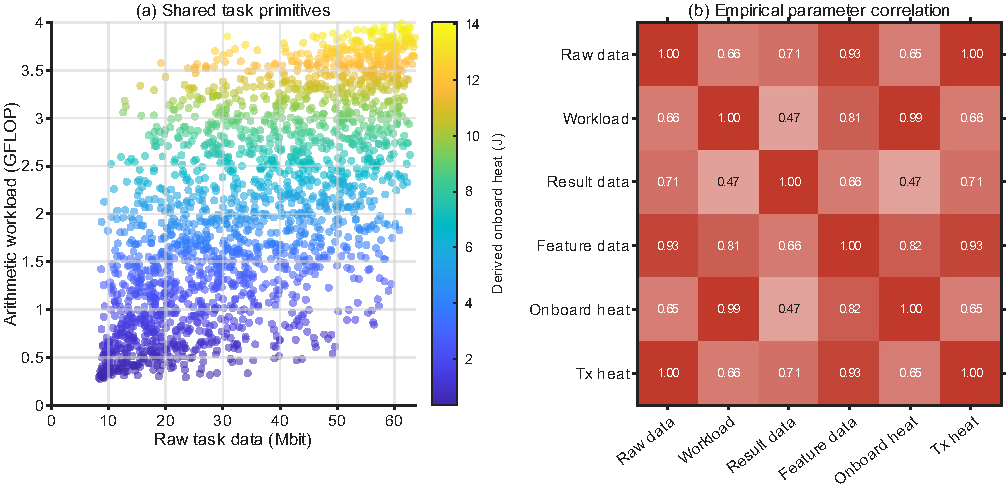
\includegraphics[width=0.98\textwidth]{figures/fig_physical_generator.pdf}
\caption{Physical-consistency audit of the revised generator. (a) A legibility sample of 2,000 of 20,000 tasks; color encodes heat derived from compute energy. (b) Correlations computed from all 20,000 tasks. No fitted flight distribution is implied.}
\label{fig:physical}
\end{figure}

\section{Sequential Scheduling Formulation}
\label{sec:mdp}

\subsection{State and transition}

The normalized 21-dimensional state is
\begin{equation}
s_t=[x_t,z_t],\qquad z_t=[h_t,e_t,q_t,u_t,b_t,\tau_t],
\end{equation}
where $x_t\in\R^{15}$ contains the task inputs used in Eqs.~\eqref{eq:onboard}--\eqref{eq:hybrid}. The six resource variables denote normalized heat, remaining energy, queue occupancy, compute utilization, bandwidth, and contact duration.

Executing action $a_t$ changes resources before the next exogenous task arrives. The implemented transition is
\begin{align}
h_{t+1}&=\clip(0.86h_t+0.17c\widehat Q_t^{(a_t)},0,1.3),\notag\\
e_{t+1}&=\clip(e_t+0.006-c\Delta e_t^{(a_t)},0,1),\notag\\
q_{t+1}&=\clip(q_t+c(\Delta q_t^{(a_t)}-\mu_t^{(a_t)}),0,1.3),\notag\\
u_{t+1}&=\clip(0.68u_t+0.32c\widehat w_t^{(a_t)},0,1.2),\notag\\
b_{t+1}&=\clip(\bar b_{t+1}-c\ell_t^{(a_t)},0.08,1),\notag\\
\tau_{t+1}&=\clip(\bar\tau_{t+1}-0.10c\widehat B_t^{(a_t)},0.05,1).
\label{eq:transition}
\end{align}
Here $\widehat Q$, $\widehat w$, and $\widehat B$ are normalized action-specific heat, work, and data demands. The terms $\Delta e$, $\Delta q$, $\mu$, and $\ell$ denote deterministic resource-use, queue, service, and link-occupation functions. Their implementations are provided with the simulator. Exogenous link variables $\bar b$ and $\bar\tau$ are sampled before each episode. Coupling $c=0$ removes action-dependent carryover, $c=0.5$ weakens it, and $c=1$ defines full coupling.

\subsection{Reward and standard DQN backbone}

The reward is the negative immediate cost plus post-decision feasibility penalties:
\begin{align}
r_t={}&-c_t^{imm}-c\big[12(h_{t+1}-0.78)_+ +15(0.18-e_{t+1})_+\notag\\
&+8(q_{t+1}-0.75)_+ +10\mathbf 1_{a_t\ne\alpha_s}(0.14-\tau_t)_+\big].
\label{eq:reward}
\end{align}
The DQN uses the unmodified factual target
\begin{equation}
y_t=r_t+\gamma(1-d_t)\max_{a'}Q_{\bar\theta}(s_{t+1},a'),
\label{eq:factual}
\end{equation}
and factual loss
\begin{equation}
L_{DQN}=\mathcal H\big(Q_\theta(s_t,a_t),y_t\big),
\end{equation}
where $\mathcal H$ denotes the Huber loss. The target network both selects and evaluates the maximizing action, as required by standard DQN.

\section{Model-Driven Counterfactual Bellman Advantage Distillation}
\label{sec:method}

The proposed method preserves the factual DQN path and adds one training-only auxiliary path. This path first supplies targets for unexecuted actions, then removes their shared within-state offset. The two stages separate the contribution of full-action supervision from the contribution of centering.

\subsection{Side-effect-free full-action preview}

For every replayed factual state, the analytical transition evaluates each $a\in\mathcal A$:
\begin{equation}
(\tilde \ell_{t,a},\tilde z'_{t,a})=F_{preview}(x_t,z_t,a).
\end{equation}
Here $\tilde \ell_{t,a}$ contains the immediate cost and post-decision feasibility penalty for action $a$. The preview does not advance time, mutate state, alter trajectories, or consume random numbers. It also reads no task beyond $x_{t+1}$. All alternatives share that next task and the exogenous link trace. The counterfactual next state therefore replaces only the six endogenous resource coordinates:
\begin{equation}
\tilde s'_{t,a}=[x_{t+1},\tilde z'_{t,a}].
\end{equation}
Evaluation and deployment never call the preview interface.

\subsection{All-action counterfactual Bellman targets}

The exact one-step outcome yields
\begin{equation}
\tilde y_{t,a}=-\tilde \ell_{t,a}+\gamma(1-d_t)
\max_{a'}Q_{\bar\theta}(\tilde s'_{t,a},a').
\label{eq:cf_target}
\end{equation}
The full-action counterfactual Bellman augmentation (CFBA) ablation fits the two unexecuted actions without centering:
\begin{align}
L_{abs}&=\frac{1}{|\mathcal A|-1}
\sum_{a\ne a_t}\mathcal H(Q_\theta(s_t,a),\tilde y_{t,a}),\notag\\
L_{CFBA}&=L_{DQN}+\lambda L_{abs}.
\label{eq:cfba}
\end{align}
CFBA isolates the value of exact full-action supervision. It creates no multi-step rollout and inserts no counterfactual transition into replay.

\subsection{Centered advantage distillation}

Absolute targets in Eq.~\eqref{eq:cf_target} share a bootstrapped state-value offset. Deployment selects $\arg\max_a Q(s,a)$, so a common additive offset cannot change the action. We define predicted and target centered advantages as
\begin{align}
\widehat A_{t,a}&=Q_\theta(s_t,a)-\frac{1}{|\mathcal A|}\sum_jQ_\theta(s_t,j),\notag\\
\tilde A_{t,a}&=\tilde y_{t,a}-\frac{1}{|\mathcal A|}\sum_j\tilde y_{t,j}.
\label{eq:center}
\end{align}
The advantage and total losses are
\begin{align}
L_{adv}&=\frac{1}{|\mathcal A|}
\sum_{a\in\mathcal A}\mathcal H(\widehat A_{t,a},\tilde A_{t,a}),\notag\\
L_{CBAD}&=L_{DQN}+\lambda L_{adv}.
\label{eq:cbad}
\end{align}
The factual term anchors the absolute Q scale, while $L_{adv}$ teaches all action gaps. The only added algorithmic hyperparameter is $\lambda$.

\begin{figure}[H]
\centering
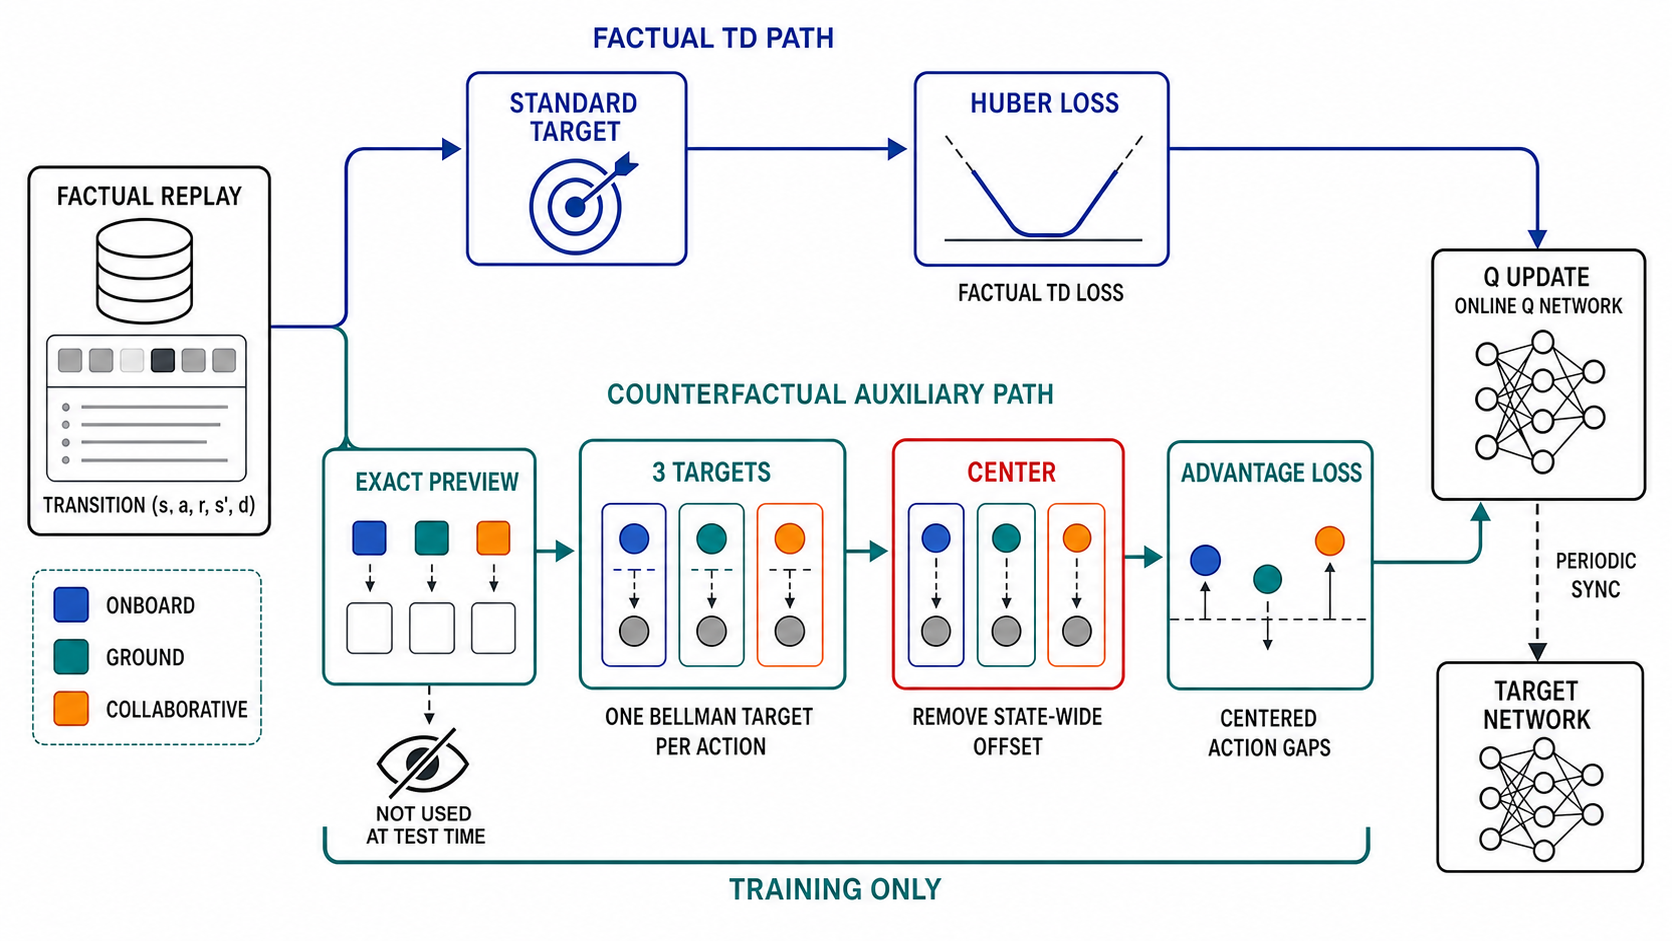
\includegraphics[width=0.98\textwidth,height=0.43\textheight,keepaspectratio]{figures/ai/fig_cbad_mechanism_arial.png}
\caption{Training-only CBAD mechanism. The upper path retains the factual standard-DQN target and Huber loss. The lower path previews all three actions, constructs three Bellman targets, centers them within state, and distills their relative advantages. Both losses update the online Q-network; the target network is synchronized only at the shared fixed interval. Preview outputs are unavailable during evaluation and deployment.}
\label{fig:mechanism}
\end{figure}

\begin{figure}[H]
\centering
\fbox{\begin{minipage}{0.93\textwidth}
\textbf{Algorithm 1: Pure-DQN training with CBAD}
\begin{enumerate}[leftmargin=1.6em,itemsep=2pt,topsep=4pt]
\item Initialize uniform replay $\mathcal D$, online $Q_\theta$, and target $Q_{\bar\theta}\leftarrow Q_\theta$.
\item At each real step, observe $s_t$ and preview $(\tilde \ell_{t,a},\tilde z'_{t,a})$ for all actions without side effects.
\item Select $a_t$ by the shared epsilon-greedy schedule, execute it once, and store the factual tuple plus previews.
\item When an update is due, sample one uniform mini-batch, compute the factual loss, compute Eqs.~\eqref{eq:cf_target} and \eqref{eq:center}, and update $\theta$ using Eq.~\eqref{eq:cbad}.
\item Synchronize $Q_{\bar\theta}$ at the shared fixed interval.
\end{enumerate}
\end{minipage}}
\par\smallskip
\caption*{Training previews are never used for evaluation or deployment.}
\label{alg:cbad}
\end{figure}

\section{Experimental Design and Settings}
\label{sec:experiments}

\subsection{Design principles}

The design separates three questions. Standard DQN versus CFBA tests whether exact targets for unexecuted actions improve learning. CFBA versus CBAD tests whether within-state centering adds value. Coupling controls test whether long-horizon learning remains useful after delayed resource effects are weakened or removed.

Standard DQN, CFBA, and CBAD share every component except the auxiliary objective. They use the same input, network, target, replay, exploration, optimizer, update cadence, target synchronization, and gradient clipping. The implementation excludes Double DQN, dueling networks, prioritized replay, multi-step returns, noisy networks, and distributional value learning.

Calibration and confirmation use disjoint model seeds and test-trace namespaces. Calibration considered $\lambda\in\{0.1,0.3,1,3\}$ with model seeds 700--703. It selected and locked $\lambda=0.3$. Confirmation used seeds 800--804 without post hoc removal, replacement, or selection. Every learned policy was trained only on the nominal $c=1$ distribution.

\begin{figure}[!htbp]
\centering
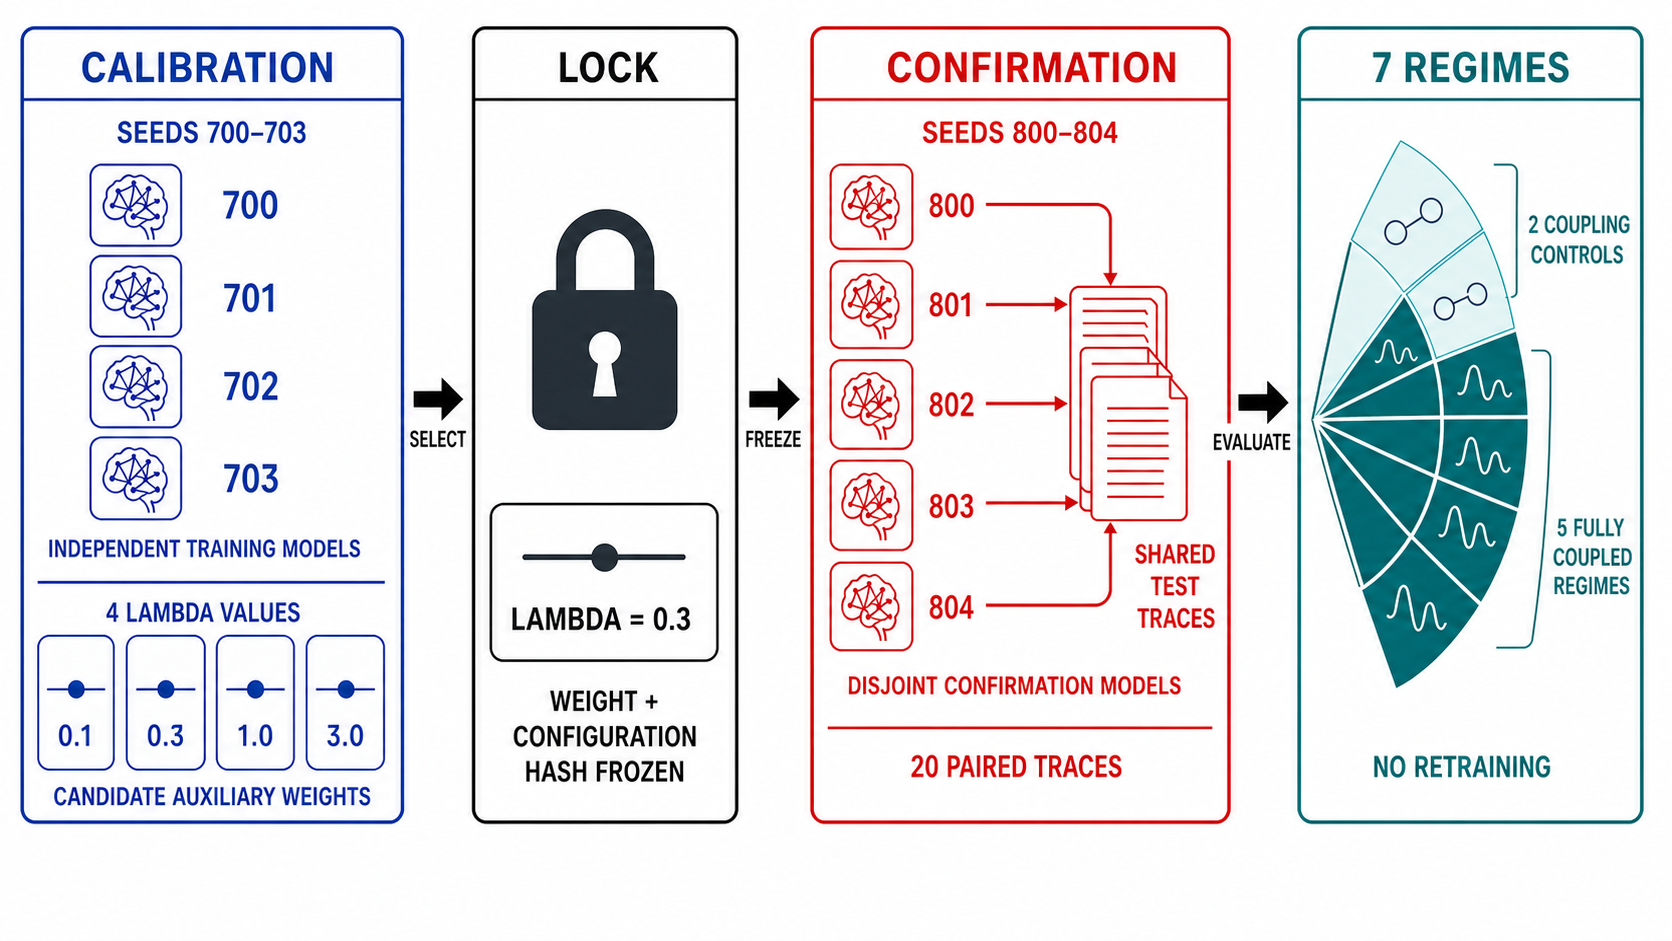
\includegraphics[width=0.98\textwidth,height=0.42\textheight,keepaspectratio]{figures/ai/fig_experiment_protocol_arial.png}
\caption{Locked calibration-confirmation protocol. Four calibration seeds compare $\lambda\in\{0.1,0.3,1.0,3.0\}$, after which $\lambda=0.3$ and the configuration are frozen. Five disjoint confirmation seeds are each evaluated on 20 paired traces in seven regimes, with no retraining or confirmatory tuning.}
\label{fig:protocol}
\end{figure}

\subsection{Training configuration}

Each network has 21 inputs, hidden widths 128--128--64, ReLU activations, and three outputs. Every model receives 600 episodes of 64 tasks, totaling 38,400 real interactions. Fixed settings are $\gamma=0.97$, learning rate $3\times10^{-4}$, batch size 128, replay capacity 100,000, and gradient-norm limit 10. Training begins after 128 transitions and performs one update every four interactions. The implemented schedule synchronizes the target network every 500 real interactions. Epsilon decreases linearly from 1 to 0.05 over 13,440 interactions.

The contextual bandit uses the same network, optimizer, exploration schedule, and interaction budget, with $\gamma=0$. It therefore learns the modeled one-step reward without a long-horizon Bellman term. Uniform replay stores only one-step factual transitions, with preview outputs attached as auxiliary training data.

All reported reviewer-revision experiments use the physically coupled generator described above. Link bandwidth and contact follow bounded noisy periodic traces generated at reset. Burst and thermal-stress episodes multiply raw data and workload by 1.45 during one contiguous interval; all dependent heat, energy, latency, and transmission quantities are recomputed from those primitives. The original independently sampled generator is retained only as a historical reproducibility mode and is not used for the revised results.

\subsection{Seven evaluation regimes}

The seven regimes separate coupling controls from fully coupled operating conditions:

\begin{enumerate}[leftmargin=1.6em]
    \item \textbf{Static ($c=0$):} removes action-dependent state transitions and delayed penalties.
    \item \textbf{Reduced coupling ($c=0.5$):} halves action-dependent resource effects.
    \item \textbf{Nominal ($c=1$):} matches the fully coupled training distribution.
    \item \textbf{Burst:} increases contiguous compute and thermal demand.
    \item \textbf{Link-limited:} reduces the available bandwidth trace by 0.22 before clipping.
    \item \textbf{Energy-limited:} lowers initial energy from 0.88 to 0.62.
    \item \textbf{Thermal-stress:} raises initial heat from 0.22 to 0.42 and includes the burst interval.
\end{enumerate}

The first two regimes control temporal coupling. The remaining five retain full coupling. Models trained at $c=1$ are transferred to both controls without retraining. Their control performance therefore measures a boundary and transfer mismatch, rather than the best policy attainable at lower coupling.

\subsection{Planning comparator, outcomes, and inference}

The main comparison includes immediate-cost argmin, a contextual bandit, a resource-threshold heuristic, standard DQN, CFBA, \method, and an exact short-horizon model-based planner. At every real decision, the planner enumerates all $3^H$ action sequences over the next $H=4$ known tasks and link states, minimizes the discounted modeled cost with $\gamma=0.97$, executes only the first action, and replans. It is exact for this four-step perfect-forecast objective but is not a 64-step global optimum; exhaustive enumeration of the complete episode would require $3^{64}$ sequences. This comparator therefore tests whether a conventional rolling planner resolves the sequential problem at practical depth while exposing its forecast and computation assumptions. Fixed onboard and fixed ground policies serve as supplemental controls.

The primary outcome is episode total cost. Secondary outcomes are immediate cost, delayed penalty, energy use, end-to-end modeled latency, transmitted data, four violation counts, action fractions, and planner wall-clock time. Every policy uses the same 20 evaluation traces within each model seed. We first average traces within each independently trained seed. Inference then uses five paired seed-level differences, rather than treating 100 traces as independent. Two-sided 95\% percentile intervals use 10,000 paired bootstrap resamples with seed 20260829. We call an improvement statistically supported only when its interval lies entirely below zero.

\subsection{Prespecified sensitivity and training diagnostics}

Without retraining or selecting models, the nominal evaluation was repeated under eight profiles: the reference configuration; compute demand $\pm20\%$; raw data volume $\pm20\%$; energy use $+20\%$; heat load $+20\%$; and link capacity $-20\%$. Each profile retained the same five models, 20 paired traces per seed, and bootstrap rule. Training logs record every episode for all five seeds. Curves report a causal 25-episode moving mean and seed-level mean $\pm$ SD for total cost, energy use, latency, and delayed penalty. These diagnostics describe optimization trajectories; confirmation claims remain based on held-out traces.

\section{Results}
\label{sec:results}

\subsection{Physical consistency preserves the CBAD--DQN effect}

Table~\ref{tab:main} and Fig.~\ref{fig:seven} summarize the revised primary outcome. Values are mean $\pm$ SD across five independent model seeds after averaging 20 shared traces within each seed.

\begin{table}[H]
\centering
\caption{Episode total cost under the physically coupled generator. MPC-4 is exact only for its stated four-step perfect-forecast objective. Lower is better; bold marks the lowest mean.}
\label{tab:main}
\resizebox{\textwidth}{!}{\begin{tabular}{lrrrrrr}
\toprule
Regime & Argmin & MPC-4 & Bandit & Threshold & DQN & CBAD \\
\midrule
Static ($c=0$) & \textbf{24.55 $\pm$ 0.21} & \textbf{24.55 $\pm$ 0.21} & 24.69 $\pm$ 0.20 & 24.74 $\pm$ 0.25 & 27.46 $\pm$ 1.34 & 27.43 $\pm$ 1.00 \\
Reduced ($c=0.5$) & 26.65 $\pm$ 0.63 & \textbf{25.70 $\pm$ 0.26} & 26.04 $\pm$ 0.37 & 26.43 $\pm$ 0.38 & 28.01 $\pm$ 0.72 & 27.80 $\pm$ 0.55 \\
Nominal & 193.42 $\pm$ 8.33 & 90.83 $\pm$ 1.71 & 100.63 $\pm$ 3.11 & 188.08 $\pm$ 6.41 & 78.80 $\pm$ 2.46 & \textbf{77.45 $\pm$ 1.86} \\
Burst & 241.20 $\pm$ 6.84 & 108.35 $\pm$ 1.99 & 129.31 $\pm$ 8.08 & 238.74 $\pm$ 6.56 & 97.99 $\pm$ 2.45 & \textbf{96.95 $\pm$ 2.12} \\
Link-limited & 272.02 $\pm$ 7.98 & 115.73 $\pm$ 1.92 & 137.55 $\pm$ 5.87 & 227.25 $\pm$ 8.36 & 102.86 $\pm$ 1.93 & \textbf{101.96 $\pm$ 1.97} \\
Energy-limited & 225.31 $\pm$ 7.73 & 126.00 $\pm$ 1.58 & 134.57 $\pm$ 2.93 & 246.46 $\pm$ 6.45 & 119.60 $\pm$ 2.42 & \textbf{118.15 $\pm$ 1.68} \\
Thermal-stress & 247.58 $\pm$ 6.25 & 109.20 $\pm$ 2.01 & 130.34 $\pm$ 7.81 & 241.80 $\pm$ 6.26 & 98.19 $\pm$ 2.46 & \textbf{97.20 $\pm$ 2.16} \\
\bottomrule
\end{tabular}}
\end{table}

\begin{figure}[H]
\centering
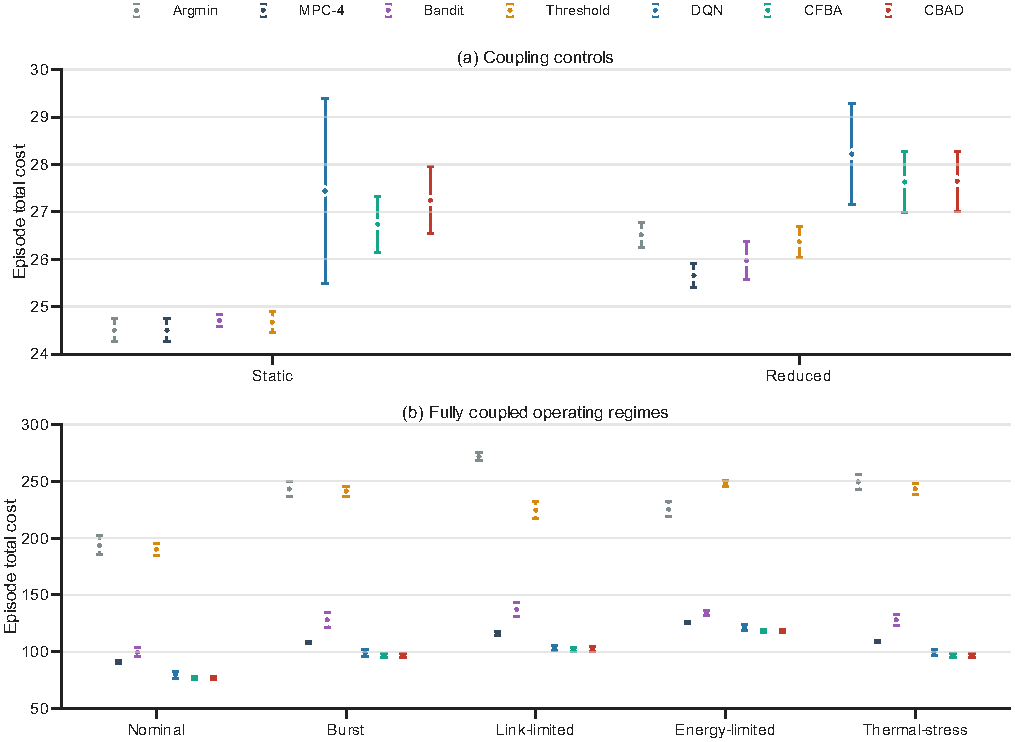
\includegraphics[width=0.98\textwidth]{figures/fig_reviewer_primary.pdf}
\caption{Seven-regime performance under physically coupled task generation. Error bars are SD across five model seeds after within-seed trace averaging. The ordinate changes between the coupling-control and fully coupled panels.}
\label{fig:seven}
\end{figure}

Across the five fully coupled regimes, \method reduced standard-DQN cost by \PhysicalCBADMinPct--\PhysicalCBADMaxPct, and every paired 95\% interval lay below zero. Nominal mean cost decreased from \PhysicalNominalDQNCost for standard DQN to \PhysicalNominalCBADCost for CBAD. This replication changes both the task generator and model training, so it is a new physical-consistency experiment rather than a re-labeling of the earlier independent-range simulation.

At $c=0$, immediate argmin and MPC-4 were identical because actions had no delayed effect. At $c=0.5$, MPC-4 had the lowest mean. In contrast, CBAD outperformed MPC-4 in all five fully coupled regimes. Nominal MPC-4 cost was \MPCNominalCost, despite perfect four-task forecasts, and planning required \MPCNominalPlanningMs{} ms per decision on the evaluation workstation. The result does not prove global superiority to planning; it shows that a four-step rolling objective misses resource consequences that the learned 64-step return can encode.

\subsection{Full-action supervision is supported; centering is not isolated}

\begin{table}[H]
\centering
\caption{Seed-paired ablation in the five fully coupled regimes under the physical generator. ``Supported'' denotes a 95\% paired bootstrap interval entirely below zero.}
\label{tab:ablation}
\resizebox{0.93\textwidth}{!}{\begin{tabular}{llrrr}
\toprule
Regime & Comparison & Mean difference & 95\% interval & Supported \\
\midrule
Nominal & CFBA $-$ DQN & -2.68 & [-4.52, -1.03] & yes \\
Nominal & CBAD $-$ CFBA & -0.02 & [-0.26, 0.22] & no \\
Nominal & CBAD $-$ DQN & -2.70 & [-4.23, -1.14] & yes \\
Burst & CFBA $-$ DQN & -2.44 & [-3.90, -0.87] & yes \\
Burst & CBAD $-$ CFBA & 0.08 & [-0.21, 0.37] & no \\
Burst & CBAD $-$ DQN & -2.36 & [-3.59, -1.04] & yes \\
Link-limited & CFBA $-$ DQN & -1.57 & [-2.78, -0.36] & yes \\
Link-limited & CBAD $-$ CFBA & 0.50 & [-0.37, 1.26] & no \\
Link-limited & CBAD $-$ DQN & -1.07 & [-2.11, -0.35] & yes \\
Energy-limited & CFBA $-$ DQN & -3.37 & [-5.48, -1.31] & yes \\
Energy-limited & CBAD $-$ CFBA & 0.14 & [-0.13, 0.41] & no \\
Energy-limited & CBAD $-$ DQN & -3.23 & [-5.05, -1.41] & yes \\
Thermal-stress & CFBA $-$ DQN & -2.42 & [-3.91, -0.95] & yes \\
Thermal-stress & CBAD $-$ CFBA & 0.08 & [-0.26, 0.42] & no \\
Thermal-stress & CBAD $-$ DQN & -2.34 & [-3.57, -0.97] & yes \\
\bottomrule
\end{tabular}}
\end{table}

Both CFBA and CBAD reduced standard-DQN cost in all five fully coupled regimes. However, CBAD--CFBA intervals crossed zero in all five regimes (\CenteringSupportedCount{} of five supported). CFBA had slightly lower means in four regimes, while CBAD was lower nominally by 0.02. Thus, the physical-consistency study supports the primary contribution of all-action counterfactual supervision but does not identify an independent centering advantage. The earlier link-limited centering effect is therefore generator-dependent and has been removed from the general claim.

\subsection{Training diagnostics show stabilization of cost, energy, and latency}

\begin{figure}[H]
\centering
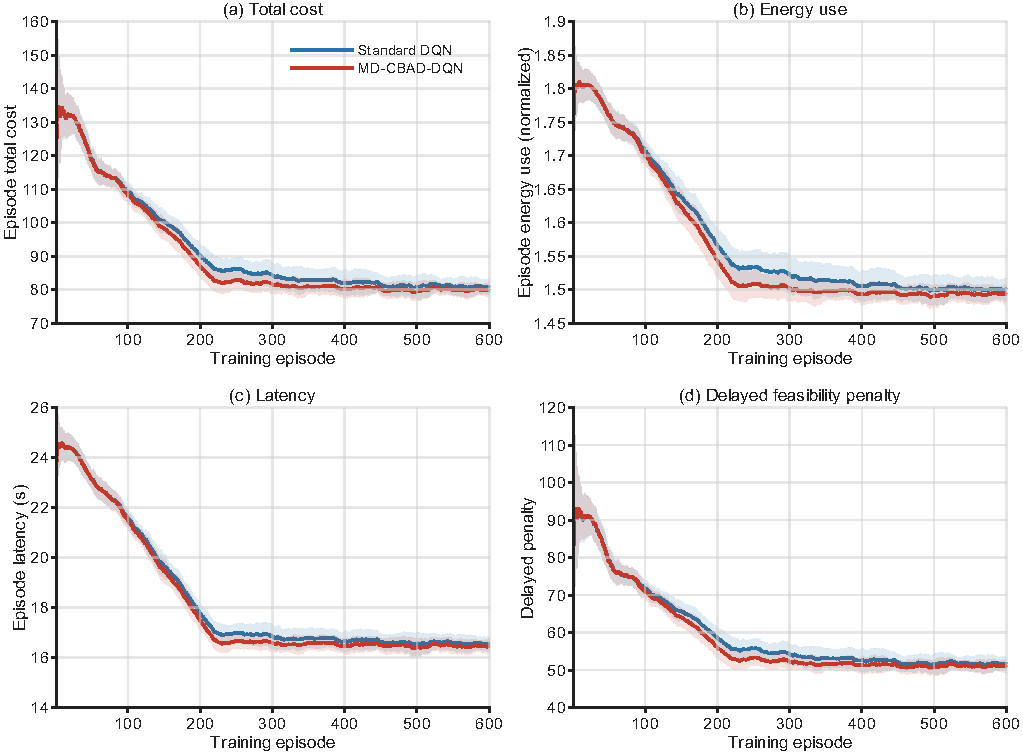
\includegraphics[width=0.98\textwidth]{figures/fig_training_diagnostics.pdf}
\caption{Training diagnostics for standard DQN and \method. Lines are means across five model seeds after a causal 25-episode moving average; shaded regions are $\pm$1 SD. Curves describe the training distribution and are not used as independent test observations.}
\label{fig:training}
\end{figure}

All four logged quantities declined rapidly during the first approximately 220 episodes and then fluctuated around a stable range (Fig.~\ref{fig:training}). Over episodes 501--600, CBAD averaged 80.48 total cost, 1.497 normalized energy use, 16.52 s latency, and a lower delayed penalty than standard DQN. These curves answer the optimization question without reintroducing the undefined ``accuracy'' metric. They show empirical stabilization, not mathematical convergence.

\subsection{The result is robust within the tested parameter envelope}

\begin{table}[H]
\centering
\caption{Prespecified parameter sensitivity for CBAD minus standard DQN. Negative differences favor CBAD; $n=5$ paired model seeds in each profile.}
\label{tab:sensitivity}
\resizebox{0.84\textwidth}{!}{\begin{tabular}{lrrrr}
\toprule
Parameter profile & Mean difference & 95\% interval & Improvement & Holm $p$ \\
\midrule
Reference & -1.45 & [-2.09, -0.88] & 1.84\% & 0.01546 \\
Compute demand $-20\%$ & -1.20 & [-1.68, -0.75] & 1.93\% & 0.01546 \\
Compute demand $+20\%$ & -1.65 & [-2.57, -0.90] & 1.81\% & 0.01546 \\
Input data $-20\%$ & -2.24 & [-3.57, -1.21] & 3.58\% & 0.00322 \\
Input data $+20\%$ & -0.84 & [-1.25, -0.47] & 0.95\% & 0.01546 \\
Energy use $+20\%$ & -1.25 & [-1.83, -0.76] & 1.19\% & 0.01546 \\
Heat load $+20\%$ & -1.44 & [-2.11, -0.87] & 1.83\% & 0.01546 \\
Link capacity $-20\%$ & -1.10 & [-1.55, -0.67] & 1.22\% & 0.00322 \\
\bottomrule
\end{tabular}}
\end{table}

\begin{figure}[H]
\centering
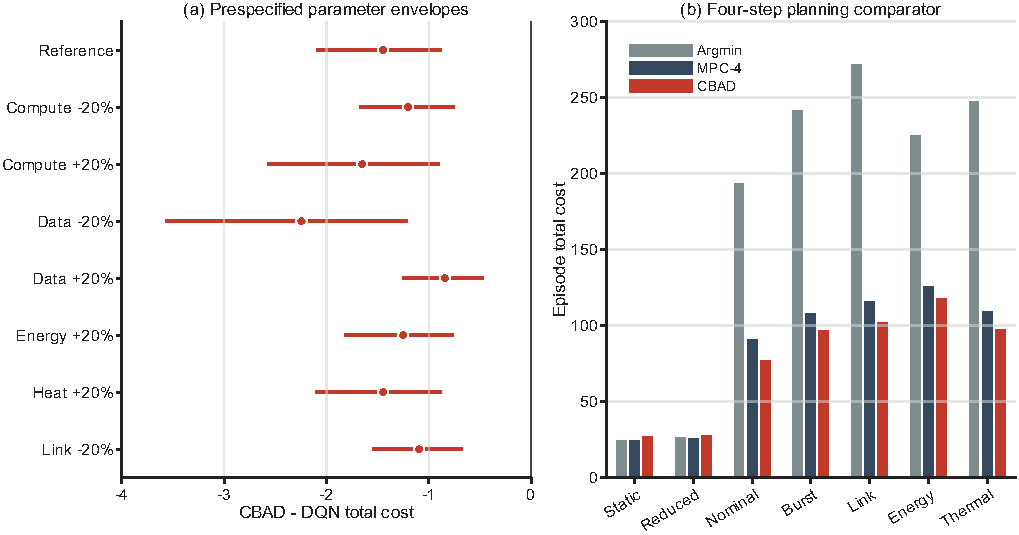
\includegraphics[width=0.98\textwidth]{figures/fig_sensitivity_planning.pdf}
\caption{Parameter robustness and planning boundary. (a) Mean paired CBAD--DQN differences with 95\% paired bootstrap intervals. (b) Immediate, four-step rolling, and learned scheduling across coupling and stress regimes.}
\label{fig:sensitivity}
\end{figure}

The CBAD--DQN interval remained below zero in all eight profiles, with relative reductions from \SensitivityMinPct{} to \SensitivityMaxPct. The largest tested effect occurred when raw data volume decreased by 20\%, whereas the smallest occurred when it increased by 20\%. This analysis supports robustness only within these prespecified one-factor envelopes; it does not validate arbitrary hardware or mission distributions.

\subsection{The learned policy adapts its action mix}

\begin{figure}[H]
\centering
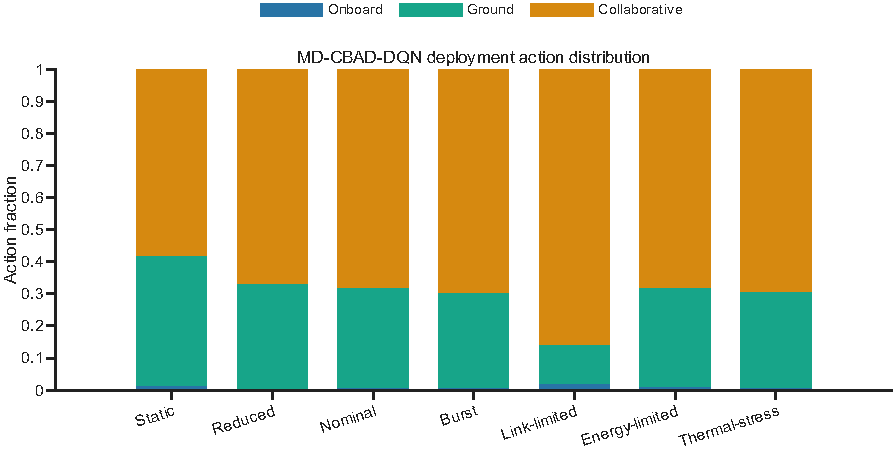
\includegraphics[width=0.90\textwidth]{figures/fig_reviewer_actions.pdf}
\caption{Mean deployment action fractions for \method under the physically coupled generator.}
\label{fig:actions}
\end{figure}

CBAD did not collapse to one processing mode. It increased onboard execution under link limitation and shifted toward ground or collaborative execution as the inherited state permitted. These action fractions are descriptive consequences of the learned policy, not additional inferential endpoints.

\section{Discussion and Limitations}

The revised evidence separates three claims. First, full-action model supervision is reproducibly useful: both CFBA and CBAD outperform the matched standard-DQN backbone across five fully coupled regimes. Second, centering is a plausible optimization device but not an independently supported source of improvement under the physical generator. Naming the complete method after centering does not license attributing the whole gain to centering; the dominant verified contribution is counterfactual Bellman supervision. Third, RL is not required for the static control. Immediate minimization is exact when action-dependent carryover is removed, and four-step receding-horizon planning is strongest under weak coupling.

The planner comparison also bounds the motivation. MPC-4 has an exact model and perfect four-task forecasts, yet a short horizon underweights consequences persisting beyond four arrivals. Increasing $H$ raises enumeration from $3^4$ to $3^H$ and may improve planning, but we did not establish the best horizon or compare against approximate tree search, mixed-integer programming, or dynamic programming with discretized resources. We therefore claim an advantage over this transparent finite-horizon baseline, not over all traditional optimization.

The new generator removes internally contradictory independent samples by deriving heat, energy, latency, and transmitted volume from common primitives. NASA and CCSDS sources bound selected engineering assumptions, while automated checks enforce data-flow inequalities. Nevertheless, the joint distribution is synthetic rather than fitted to mission telemetry. NASA itself cautions that component performance is mission-specific~\cite{nasa2026soa}. The sensitivity study covers only prespecified one-factor changes, not simultaneous uncertainty or structural model error.

Matched training components make attribution within this simulator direct, but external validity remains limited. Preview outcomes are exact by construction and may be biased onboard. The topology remains one satellite and one ground path, the action space contains only three modes, five seeds provide limited power for small incremental effects, and inference is simulation-based. Future work should use flight or hardware-in-the-loop traces, quantify preview uncertainty, expand to multiple satellites and contacts, and compare scalable approximate planning at longer horizons.

\section{Conclusion}

We introduced \method to exploit exact one-step resource models without changing the factual standard-DQN update. Under a physically coupled generator, CBAD improved on standard DQN across five fully coupled regimes and eight parameter profiles. A four-step exact rolling planner and coupling controls show that the benefit is confined to sufficiently persistent resource carryover. The revised ablation supports full-action supervision but not a separate centering effect over CFBA; this boundary is part of the result.

\section*{Funding}

This work was supported by the National Key Research and Development Program of China under Grants 2022YFF0503904 and 2022YFD2401202. Additional support came from the Shenzhen Higher Education Institutions Stabilization Support Program under Grant GXWD\allowbreak20220811163556003. The National Natural Science Foundation of China supported this work under Grant 62202127, and the Shenzhen Natural Science Foundation under Grant JCYJ\allowbreak20241202123731040. Further support came from the Guangxi Science and Technology Base and Talent Special Project under Grant Gui Ke AD25069103.

\section*{Data and Code Availability}

The simulator, model checkpoints, raw evaluations, seed-level summaries, fixed-seed bootstrap statistics, and table/figure regeneration scripts are available from the corresponding authors upon reasonable request. A permanent repository URL or DOI will replace this statement if the materials are made public before publication.

\begingroup
\small
\setlength{\itemsep}{0.2em}
\bibliographystyle{plain}
\bibliography{ref}
\endgroup

\end{document}
